\todo[inline]{Verantwortlich: Artur \\}


Diese Projektgruppe des ELISE Projektes wir dem Lehrstuhl Medizinische Informatik \& Mikrosystementwurf und dem Lehrstuhl für Mustererkennung zugeordnet. \\

Die Gruppe wird von Dr.-Ing. Armin Grünewald, David Krönert und Frédéric Li geleitet. 
Innerhalb der Gruppe wurden dazu unabhändig ein Sprecher und ein stellvertretender Sprecher von den Gruppenmitgliedern gewählt. Als Projektgruppensprecher wurde Artur Piet und als Stellvertreter Jonas Pöhler ausgewählt. 
Diese Stellung ist jedoch nicht die eines Leiters mit Entscheidungs- und Weisungsbefugnissen. Die Sprecher sind also auf die Kooperationsbereitschaft der anderen Gruppenmitglieder angewiesen. 
Konkrete Aufgaben der Sprecher waren unter anderen das Verteilen von Verantwortungsbereichen auf alle Mitglieder, die Einführung von regelmäßigen Gruppentreffen um den Überblick über alle Fortschritte zu garantieren und die Übernahme möglichst aller organisatorischer Tätigkeiten (z.B. Messreihen organisieren, Beschaffungsprozesse koordinieren, usw.). \\

Die Laufzeit der Projektgruppe wurde auf etwa 1 Jahr gesetzt, wobei das Kick-Off Meeting am 23.10.2017 stattfand. Der geforderte individuelle Zeitaufwand aller Gruppenmitglieder entspricht der jeweils im Modulhandbuch des Studienganges definierten Leistungspunkte für die Projektarbeit, also 600 Stunden für Jonas Pöhler, Arnaud Eric Toham Waffo, Boris Kamdem, Kevin Orth, Meryem Dural sowie Minas Michail und 270 Stunden für Artur Piet. Es folgt ein Balkendiagramm mit den geforderten Stunden im Verlgeich zum tatsälichem Zeitaufwand. \\


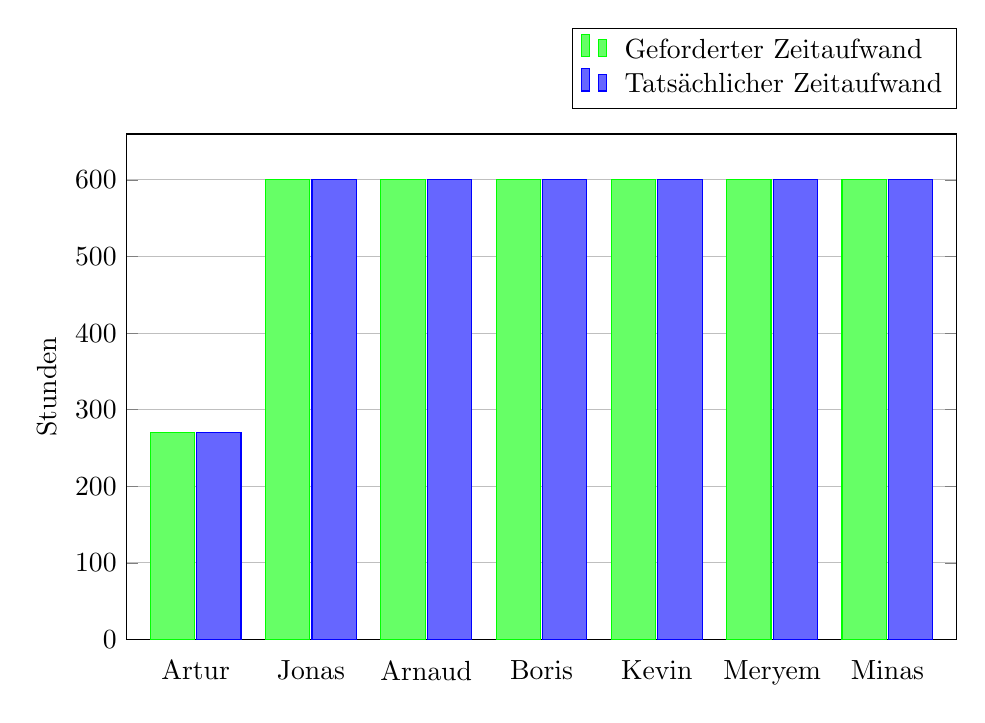
\begin{tikzpicture}
    \begin{axis}[
        width  = \textwidth,
        height = 8cm,
        major x tick style = transparent,
        ybar=2*\pgflinewidth,
        bar width=16pt,
        ymajorgrids = true,
        ylabel = {Stunden},
        symbolic x coords={Artur,Jonas,Arnaud,Boris,Kevin,Meryem,Minas},
        xtick = data,
        scaled y ticks = false,
        enlarge x limits=0.1,
        ymin=0,
        legend cell align=left,
        legend style={
                at={(1,1.05)},
                anchor=south east,
                column sep=1ex
        }
    ]
        \addplot[style={green,fill=green!60,mark=none}]
            coordinates {(Artur, 270) (Jonas,600) (Arnaud,600) (Boris,600) (Kevin,600) (Meryem,600) (Minas,600)};

        \addplot[style={blue,fill=blue!60,mark=none}]
             coordinates {(Artur,270) (Jonas,600) (Arnaud,600) (Boris,600) (Kevin,600) (Meryem,600) (Minas,600)};

        \legend{Geforderter Zeitaufwand,Tatsächlicher Zeitaufwand}
    \end{axis}
\end{tikzpicture}



\subsection{Verantwortungsbereiche}
Innerhalb der Projektgruppe (PG) war ein Ziel, dass jeder der Mitglieder "Experte" für einen Bereich wird. Damit haben wir die Verantwortung relativ gleichmäßig auf alle aufgeteilt. Dazu muss noch erwähnt werden, dass die Teammitglieder nicht nur ausschließlich die Aufgaben des jeweiligen Verantwortungsbereiches erlegibt habe. Es wurde sich vielmehr gegenseitig immer unterstützt und viel zusammengearbeitet. Die Verantwortungsbereiche haben sich mit der Zeit folgendermaßen aufgeteilt: \\

$ \bullet $ Artur Piet: Mustererkennung, 3D-Konstruktion und Sprecher der PG \\
$ \bullet $ Jonas Pöhler: Hardware, Webanbindung und Stellv. Sprecher der PG \\
$ \bullet $ Arnaud Eric Toham Waffo: Elektrodenauswahl \\
$ \bullet $ Boris Kamdem: Langeweile-Szenario und Fragebogen in VR \\
$ \bullet $ Kevin Orth: Komplette Hardware \\
$ \bullet $ Meryem Dural: Frustations-Szenario in VR \\
$ \bullet $ Minas Michail: Glücks-Szenario in VR \\




%\begin{table}[h]
%\begin{tabular}{lllll} 
%\begin{tikzpicture}[scale=0.62]\tikzset{lines/.style={draw=black},}\pie{73/,13/,7/,7/}\end{tikzpicture} &
%\begin{tikzpicture}[scale=0.62]\tikzset{lines/.style={draw=black},}\pie{73/,13/,7/,7/}\end{tikzpicture} &
%\begin{tikzpicture}[scale=0.62]\tikzset{lines/.style={draw=black},}\pie{73/,13/,7/,7/}\end{tikzpicture} &
%\begin{tikzpicture}[scale=0.62]\tikzset{lines/.style={draw=black},}\pie{73/,13/,7/,7/}\end{tikzpicture} &  \\
%\begin{tikzpicture}[scale=0.62]\tikzset{lines/.style={draw=black},}\pie{73/,13/,7/,7/}\end{tikzpicture} &
%\begin{tikzpicture}[scale=0.62]\tikzset{lines/.style={draw=black},}\pie{73/,13/,7/,7/}\end{tikzpicture} &
%\begin{tikzpicture}[scale=0.62]\tikzset{lines/.style={draw=black},}\pie{73/,13/,7/,7/}\end{tikzpicture} &
%LEGEND & \\
%\end{tabular}
%\end{table}

\subsection{Gruppentreffen}
Die wöchentliche Gruppentreffen finden immer Donnerstags ab 14:00 Uhr statt und beginnen in der Regel mit einer Update-Runde. Hierbei kommen alle Gruppenteilnehmer der Reihe nach dran und jeder erklärt kurz woran letzte Woche gearbeitet wurde, was die aktuellen Herausfoderungen und Probleme sind und was genau als nächstes geplant ist. Ziel ist es den Austausch und die Kommunikation unter den Teammitgliedern und den Projektleitern zu fördern, damit alle Teilnehmer auf dem selben Wissenstand sind, da einzelnen Aufgaben durchaus großen Einfluß auf Tätigkeiten von anderen Mitgliedern haben können. \\